% Contributors: Kevin Wu, Emily Jin
\section{The \emph{k}-means problem}
The $k$-means optimization problem is defined as:
\begin{enumerate}
\item \underline{Input}: A set of $n$ points $\mathcal{S} = x_1,....x_n \in
\mathbb{R}^d$ and a positive integer $k<n$.
\item \underline{Output}: $T \subset  \mathbb{R}^d$ s.t. $|T|=k$. 
\item \underline{Goal}: minimize ``cost'' of $T$ where: $cost(T) 
:= \sum_{i = 1}^{n} \min_{\mu_j \in T} \norm{x_i-\mu_j}^2 $.
\end{enumerate}

Note that unlike the $k$-centers or $k$-medians problem, the $k$-means problem (as defined above) requires that the set of input points belong to a \emph{Euclidean} space as opposed to a metric space; later we will define a generalized $k$-means problem setup for which $x_1,....x_n$ may come from any metric space. \\

\noindent\textbf{Approximate solutions for $k$-means:}  

As before, we can attempt an exhaustive search with exponential
time complexity. If we want some solution in polynomial time, however, we
must settle for an approximation, as $k$-means is also an NP-hard
optimization problem. \\

(The statement regarding NP-hardness of $k$-means assumes that $d$ in $\mathbb{R}^d$ must be greater than or equal to 2; when $d = 1$, the problem is actually solvable in polynomial time using dynamic programming).\\

One approximate solution is Lloyd's method for $k$-means, which alternates between optimizing cluster assignments and cluster centers until some stopping criterion (i.e. convergence of cluster centers $\vec{\mu}$).

\begin{algorithm}
\caption{Lloyd's Algorithm:}
\begin{algorithmic} 
\STATE Pick randomly $x_1,...,x_k $ from $\mathcal{X}$ \;
\WHILE{stopping criteria not satisfied}
\STATE Assign points of the dataset to the closest center \;
\FORALL {clusters $C_1, ..., C_k$\;}
\STATE Compute the new centroid $\mu_j = \frac{1}{|C_j|}
\sum_{x_i\in C_j} x_i$, $\forall j \in \{1,...,k\}$\;
\ENDFOR
\ENDWHILE
\end{algorithmic}
\end{algorithm}

\begin{remark}
Call $cost(T^*)$ the cost of the optimal k-means solution, and $cost(T^{LLOYD})$ the cost the approximate solution returned by k-means. Then necessarily, $cost(T^{LLOYD}) \geq cost(T^*)$.
\end{remark}

\begin{example} Consider the following setting and dataset
where $k=2$ and $d=1$:
\begin{figure}
    \centering
    \captionsetup{width=0.8\textwidth}
    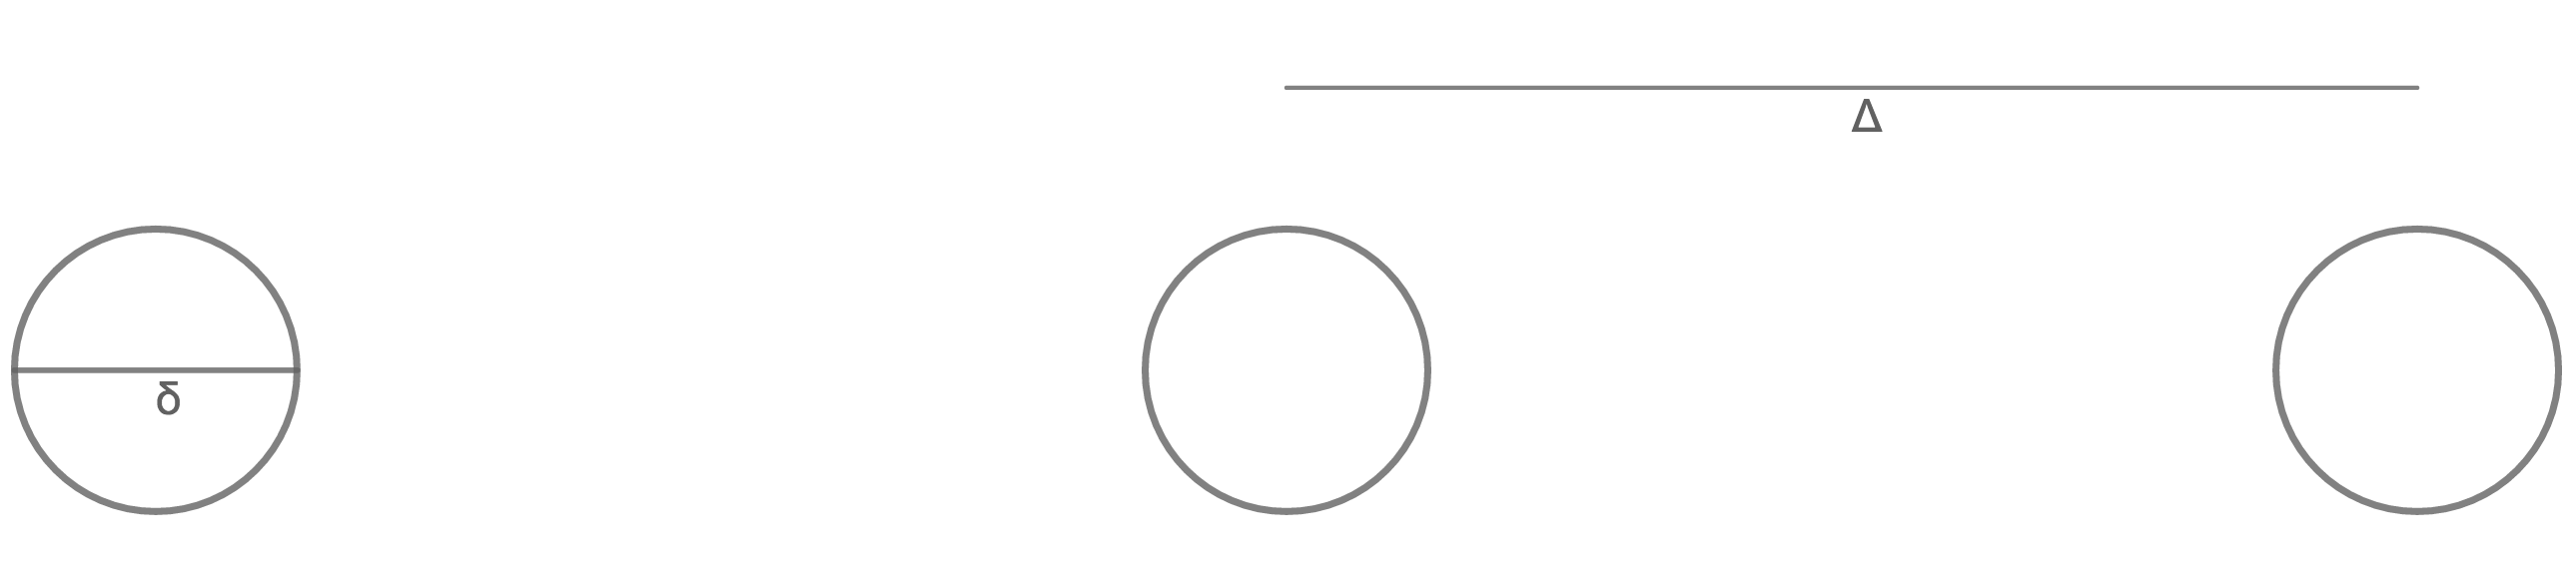
\includegraphics[scale=0.4]{chapter_1/files/kmeans.png}
    \caption{An example of datapoints and initial setting where
    Lloyd's algorithm fails to be optimal.}
    \label{fig:kmeans}
\end{figure}

The dashed lines point to the current cluster centers, with 0
for the blue cluster and 28 for the red cluster. On this
setting, Lloyd's algorithm makes no further improvement (it
terminates after one iteration), since the middle point at 16
is closer to the red cluster center 28 than to the blue cluster
center 0. And the total cost is $0^2+12^2+12^2=288$.

However, the optimal cluster center assignment should be 8 for
the blue cluster and 40 for the red cluster, which gives a cost
of $8^2+8^2+0^2=128$. Thus, Lloyd's algorithm does not give the
optimal solution.
\end{example}

\begin{remark}
$cost(T^{LLOYD})$ is unbounded and may be \emph{arbitrarily bad} compared to the optimal solution depending on the initialization of cluster means.
\end{remark}

\begin{example} 
Insert example from 9/24 class.  
\end{example}




